---
title: "泛函分析作业251008"
date: 2025-10-08
collections: "泛函分析作业"
tags: ["泛函分析"]
categories: ["泛函分析"]
---
\problem[1.4.1]在二维空间 $\mathbb{R}^2$ 中, 对每一点 $z = (x, y)$, 令
\begin{align*}
	\|z\|_1 &= |x| + |y|; & \|z\|_2 &= \sqrt{x^2 + y^2}; \\
	\|z\|_3 &= \max(|x|, |y|); & \|z\|_4 &= (x^4 + y^4)^{\frac{1}{4}}.
\end{align*}

(1) 求证 $\|\cdot\|_i$ ($i=1,2,3,4$) 都是 $\mathbb{R}^2$ 的范数.

(2) 画出 $(\mathbb{R}^2, \|\cdot\|_i)$ ($i=1,2,3,4$) 各空间中的单位球面图形.

(3) 在 $\mathbb{R}^2$ 中取定三点 $O = (0,0)$, $A = (1,0)$, $B = (0,1)$, 试在上述四种不同范数下求出 $\triangle OAB$ 三边的长度.

\begin{solution}
	(1) 正定性: 显然四者都是非负的, 并且当且仅当 $z=(0,0)$ 时为 0.

	齐次性: $\norm{\alpha z}_1=|\alpha x|+|\alpha y|=\alpha\norm{z_1}$, $\norm{\alpha z}_2=\sqrt{(\alpha x)^2+(\alpha y)^2}=\alpha\sqrt{x^2+y^2}=\alpha\norm{z}_2$, $\norm{\alpha z}_3=\max(|\alpha x|,|\alpha y|)=\alpha\max(|x|,|y|)=\alpha\norm{z}_3$, $\norm{\alpha z}_4=((\alpha x)^4+(\alpha y)^4)^{1/4}=\alpha (x^4+y^4)^{1/4}=\alpha\norm{z}_4$.

	三角不等式: $\norm{z_1+z_2}_1=|x_1+x_2|+|y_1+y_2|\leqslant |x_1|+|x_2|+|y_1|+|y_2|=\norm{z_1}_1+\norm{z_2}_1$, $\norm{z_1+z_2}_2=\sqrt{(x_1+x_2)^2+(y_1+y_2)^2}\leqslant \sqrt{x_1^2+y_1^2}+\sqrt{x_2^2+y_2^2}=\norm{z_1}_2+\norm{z_2}_2$, $\norm{z_1+z_2}_3=\max(|x_1+x_2|,|y_1+y_2|)\leqslant \max(|x_1|+|x_2|,|y_1|+|y_2|)\leqslant\max(|x_1|,|y_1|)+\max(|x_2|,|y_2|)=\norm{z_1}_3+\norm{z_2}_3$, $\norm{z_1+z_2}_4=((x_1+x_2)^4+(y_1+y_2)^4)^{1/4}\leqslant (x_1^4+y_1^4)^{1/4}+(x_2^4+y_2^4)^{1/4}=\norm{z_1}_4+\norm{z_2}_4$.

	(2)
	\begin{figure}[H]
		\centering
		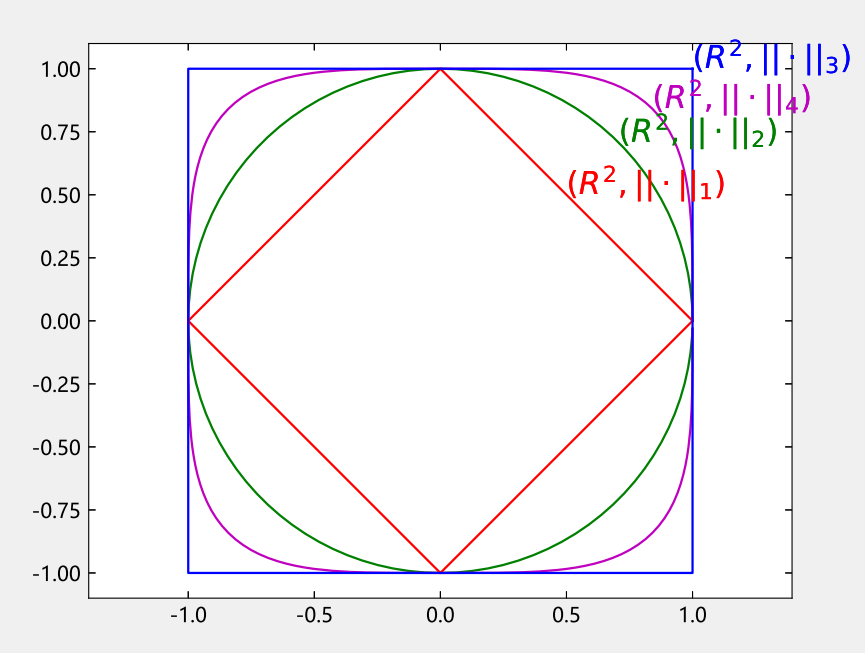
\includegraphics[width=0.6\textwidth]{figures/泛函/1.4.1}
	\end{figure}

	(3)

	$\norm\cdot_1: 4$, $\norm\cdot_2: 2+\sqrt{2}$, $\norm\cdot_3: 3$, $\norm\cdot_4: 2+\sqrt[4]{2}$.
\end{solution}

\problem[1.4.2]设 $C(0,1]$ 表示 $(0,1]$ 上连续且有界的函数 $x(t)$ 全体. 对 $\forall x \in C(0,1]$, 令 $\|x\Vert = \sup_{0 < t \leqslant 1} |x(t)|$. 求证:

(1) $\|\cdot\|$ 是 $C(0,1]$ 上的范数;

(2) $l^\infty$ 与 $C(0,1]$ 的一个子空间是等距同构的.

\begin{proof}
	(1) 正定性显然.

	齐次性 $\norm{\alpha x(t)}=\sup\limits_{0<t\leqslant 1}|\alpha x(t)|=\alpha\sup\limits_{0<t\leqslant 1}|x(t)|=\alpha\norm{x(t)}$.

	三角不等式: $\norm{x_1(t)+x_2(t)}=\sup\limits_{0<t\leqslant 1}|x_1(t)+x_2(t)|\leqslant \sup\limits_{0<t\leqslant 1}|x_1(t)|+|x_2(t)|\leqslant \sup\limits_{0<t\leqslant 1}|x_1(t)|+\sup\limits_{0<t\leqslant 1}|x_2(t)|=\norm{x_1(t)}+\norm{x_2(t)}$.

	(2) 构造映射 $T: l^\infty\to C(0,1]$, $\forall \{a_n\}\in l^\infty, T(\{a_n\})$ 表示 $x(\frac1n)=a_n$ 且用折线段连接 $x(\frac 1n),x(\frac1{n+1})$ 两点的连续函数. 显然这是个单射且像集是 $C(0,1]$ 的子集. 并且由折线段的线性性该映射是线性映射. 下面证其还保范数.

	首先对于折线段, 其最大值必取在端点处, 故 $\norm{T(\{a_n\})}=\sup x(\frac 1 n)=\sup a_n=\norm{\{a_n\}}$.

	所以 $l^\infty$ 与 $C(0,1]$ 的一个子空间 $T(l^\infty)$ 等距同构.

\end{proof}

\problem[1.4.3]在 $C^1[a,b]$ 中, 令
\[
\|f\|_1 = \left( \int_a^b (|f|^2 + |f'|^2) \, \td x \right)^{\frac{1}{2}} \quad (\forall f \in C^1[a,b]),
\]

(1) 求证 $\|\cdot\|_1$ 是 $C^1[a,b]$ 上的范数.

(2) 问 $(C^1[a,b], \|\cdot\|_1)$ 是否完备?

\begin{proof}
	(1) 正定性由连续函数性质可知. 齐次性由积分的线性性可知.

	三角不等式, 用柯西施瓦茨不等式可得 $$\int_a^b |fg|+|f'g'|\td x\leqslant \norm{f}_1\norm{g}_1$$ 从而满足.

	(2) 任取 $c\in (a,b)$, 对于函数 $f(x)=|x-c|\notin C^1[a,b]$, 但函数列 $f_n(x)=\sqrt{(x-c)^2+\frac 1n}$.

	有 $|f_n(x)-f(x)|\leqslant\sqrt{\frac1n}$, 从而 $\int_a^b |f_n(x)-f(x)|^2\td x\leqslant (b-a)\frac1n$.

	考虑 $sgn_c(x)=\left\lbrace\begin{array}{ll}
		-1,& x<c\\
		0, & x=c\\
		1, & x>c
	\end{array}\right.$, 有 $|f_n'(x)-sgn_c(x)|=|(x-c)|(\frac{1}{|x-c|}-\frac{1}{\sqrt{(x-c)^2+\frac 1 n}})$.

	从而 $\norm{f_n-f}=O(\frac{1}{\sqrt n})\to 0$. 即 $\{f_n\}$ 收敛至 $f$, 但 $f\notin C^1[a,b]$ 故不完备.
\end{proof}

\problem[1.4.4]在 $C[0,1]$ 中, 对每一个 $f \in C[0,1]$, 令
\begin{align*}
	\|f\|_1 &= \left( \int_0^1 |f(x)|^2 \, \td x \right)^{\frac{1}{2}}, \\
	\|f\|_2 &= \left( \int_0^1 (1+x) |f(x)|^2 \, \td x \right)^{\frac{1}{2}},
\end{align*}
求证: $\norm{\cdot}_1$ 和 $\norm{\cdot}_2$ 是 $C[0,1]$ 中的两个等价范数.

\begin{proof}
	由于 $1\leqslant (1+x)\leqslant 2$. 所以有
	$\norm{f}_1\leqslant\norm f_2\leqslant\sqrt{2}\norm{f}_1$.
\end{proof}

\problem[1.4.5] 设 $BC[0,\infty)$ 表示 $[0,\infty)$ 上连续且有界的函数 $f(x)$ 全体, 对于每个 $f \in BC[0,\infty)$ 及 $a > 0$, 定义
\[
\|f\|_a = \left( \int_0^\infty e^{-ax} |f(x)|^2 \, \td x \right)^{\frac{1}{2}}.
\]

(1) 求证 $\|\cdot\|_a$ 是 $BC[0,\infty)$ 上的范数.

(2) 若 $a, b > 0$, $a \neq b$, 求证 $\|\cdot\|_a$ 与 $\|\cdot\|_b$ 作为 $BC[0,\infty)$ 上的范数是不等价的.

\begin{proof}
	(1) 正定性: 结合函数的连续性可知若 $f\neq 0$, 则 $\norm{f}_a\neq 0$.

	齐次性: $\norm{\alpha f}=\left(\mint[0]^\infty e^{-ax}|\alpha f(x)|^2\td x\right)^{\frac12}=\left(\alpha^2\mint[0]^\infty e^{-ax}|f(x)|^2\td x\right)^{\frac12}=\alpha\norm{f}_a$.

	三角不等式: 由柯西-施瓦茨不等式, $$\int_0^\infty e^{-ax}|f(x)+g(x)|^2\td x\leqslant \norm{f}_a^2+\norm{g}_a^2+2\int_0^\infty e^{-ax}|f(x)||g(x)|\td x\leqslant\norm f_a^2+\norm g_a^2+2\norm f_a\norm g_a$$ 所以有 $\norm{f+g}_a\leqslant \norm{f}_a+\norm g_a$.

	(2) 不妨设 $a>b>0$ 考虑函数列

	$f_n^2=\left\lbrace\begin{array}{ll}
		0, & x\in [0,n-\frac1b]\\
		be^{bn}(x-n+\frac1b), & x\in(n-\frac1b,n]\\
		e^{bx}, & x\in (n,n+1]\\
		e^{b(n+1)}-(x-n-1)be^{b(n+1)}, & x\in (n+1,n+1+\frac 1b)\\
		0, & x\in [n+1+\frac 1b,\infty)
	\end{array}\right.$ 从 $n>\frac1b$ 开始定义.

	在 $\norm\cdot_a$ 中, $\norm{f_n}_a\leqslant \mint[n-\frac 1b]^{n+1+\frac1b}e^{(b-a)x}\td x\leqslant \frac{1}{a-b}e^{(b-a)(n-\frac1b)}$ 由于 $b<a$ 所以 $n\to\infty$ 时 $\frac{1}{a-b}e^{(b-a)(n-\frac{1}{b})}\to 0$, 即 $\norm{f_n}_a\to 0$.

	但在 $\norm\cdot_b$ 中, $\norm{f_n}_b\geqslant \mint[n]^{n+1}e^{bx-bx}\td x=1$, 从而不收敛, 故两个范数不等价.
\end{proof}

\problem[1.4.8] 记 $[a,b]$ 上次数不超过 $n$ 的多项式全体为 $\mathbb{P}_n$. 求证:
$\forall f(x) \in C[a,b], \exists P_0(x) \in \mathbb{P}_n$, 使得
\[ \max_{a \leqslant x \leqslant b} |f(x) - P_0(x)| = \min_{P \in \mathbb{P}_n} \max_{a \leqslant x \leqslant b} |f(x) - P(x)|.
\]
也就是说, 如果用所有次数不超过 $n$ 的多项式去对 $f(x)$ 一致逼近, 那么 $P_0(x)$ 是最佳的.

\begin{proof}
	由于 $C[a,b]$ 关于范数 $\norm{f}=\max\limits_{a\leqslant x\leqslant b}|f(x)|$ 构成 B 空间, $\mathbb P_n$ 是 $C[a,b]$ 的有穷维子空间 (可以取基为 $\{1,x,\ldots,x^n\}$), 所以根据最佳逼近元定理存在唯一的 $P_0(x)\in\mathbb P_n$ 使得 $\norm{P_0(x)-f(x)}=\rho(f(x),\mathbb P_n)$.
\end{proof}